\appendix
\chapter{Sound Annotation and Analysis Tool}\label{appendix:a} %Appendix

\begin{figure}
    \centering
    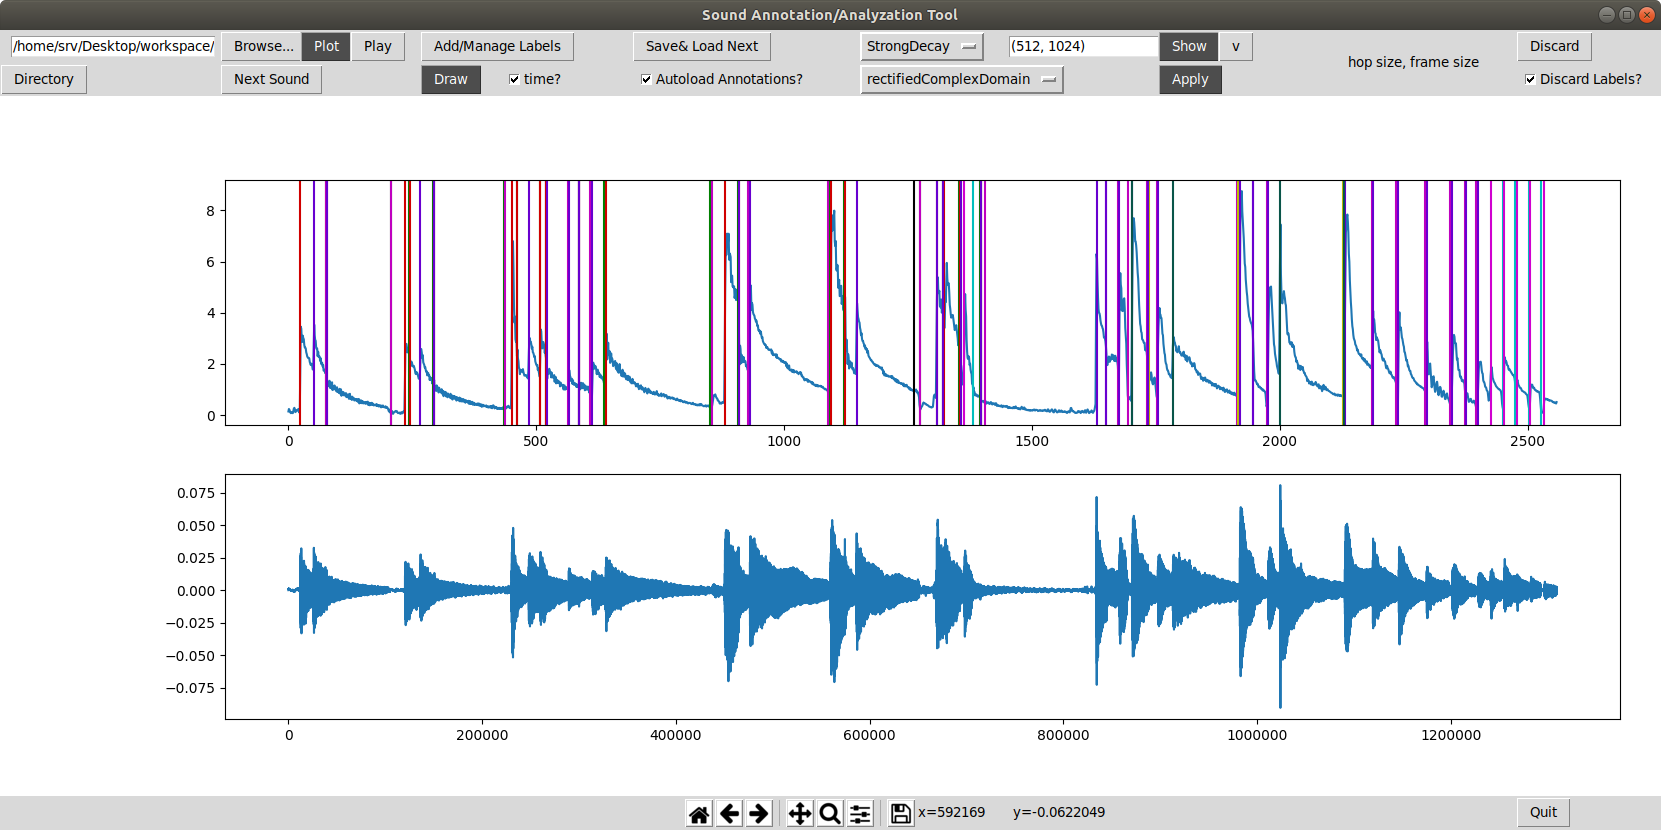
\includegraphics[width=\columnwidth]{appendix/saat.png}
    \caption{A screenshot of the Sound Annotation and Analysis Tool}
    \label{fig:saat}
\end{figure}

This tool is developed to save time on annotation and inspection of the sound files. Written in Python.

GUI: Tkinter (https://docs.python.org/3/library/tkinter.html)\\
Sound: PyAudio (https://pypi.org/project/PyAudio/)\\
Audio Features: Essentia (https://essentia.upf.edu/)\\
Onset Detection Functions: Essentia and madmom (https://pypi.org/project/madmom/)\\

Audio features from Essentia library can be extracted and plotted on the interactive frame. Interactive frame allows navigation through the plot and control the sound player. Two features can be shown at the same time. 
Onset detection functions from Essentia and madmom library can be applied to the loaded sound. Detected onsets can be saved as annotations.

\newpage

\chapter{Guitar Noises Dataset}\label{appendix:b}

Dataset is available on https://freesound.org/people/svurucu/packs/29986/.

Buzz noises are created via following procedure: String is pressed on the left side of the fret (closer to headstock) and the note is played naturally by plucking the string. Then, the string is slowly released until it produce a buzz (see \ref{buzzsection}).  \\

Slide noises are generated between two predetermined frets. The player had one second to move between each origin-destination fret pairs. Movement had to start and end inside of the one second duration. Slide noises have two versions, the string can be released or still pressed at the beginning of the slide. The latter causes a louder 'squeak' sound. Origin-destination fret pairs are selected by fixing the origin, or their distance. Then, all possible combinations are performed within the first twelve frets.

Currently, there are 36 buzz and 234 slide noises available.

\textbf{Recording Details:}

Guitar: Yamaha C80 Classical Guitar \\
Strings: D'Addario EXP45 Coated Classical Guitar Strings, Normal Tension \\
Microphone: Samson C05 (The microphone was placed 10 cm in front of the sound hole)\\
Soundcard: Focusrite Scarlett 18i20 \\
Environment: Small (6m$^2$) anechoic chamber \\